\documentclass{diploma}

\student{Шелаев Серафим Ильич}
\group{М8О-408Б-22}
\theme{Распознавание визуальных признаков детских рисунков, ассоциированных с психологическими характеристиками ребёнка, нейросетевыми методами}

\supervisor{Судаков Владимир Анатольевич}
\firstConsultant{---}
\secondConsultant{---}
\reviewer{---}

\faculty{№ 8 <<Компьютерные науки и прикладная математика>>}
\department{806}
\speciality{01.03.02 <<Прикладная математика и информатика>>}
\profile{Информатика}

\departmentFullName{№ 806}
\headOfDepartment{Крылов Сергей Сергеевич}

\date{\uline{\hspace{24pt}} мая \the\year\ года}

\newacronym{cnn}{СНС}{свёрточная нейронная сеть}

\newacronym{ml}{МО}{машинное обучение}

\newacronym{api}{API}{программный интерфейс приложения (англ.\ Application Programming Interface)}

\newacronym{rest}{REST}{Representational State Transfer --- архитектурный стиль построения веб-сервисов}

\newacronym{http}{HTTP}{Hypertext Transfer Protocol --- протокол передачи гипертекста}

\newacronym{json}{JSON}{JavaScript Object Notation --- текстовый формат обмена данными}

\newacronym{sql}{СУБД}{система управления базами данных}

\newacronym{uuid}{UUID}{Universally Unique Identifier --- универсально-уникальный идентификатор}

\newacronym{asgi}{ASGI}{Asynchronous Server Gateway Interface --- интерфейс асинхронного веб-сервера для Python}

\newacronym{tta}{TTA}{Test-Time Augmentation --- усреднение предсказаний по нескольким аугментированным версиям одного изображения}

\newacronym{clahe}{CLAHE}{Contrast Limited Adaptive Histogram Equalization --- адаптивное локальное выравнивание гистограммы с ограничением контраста}

\newacronym{mlp}{MLP}{Multi-Layer Perceptron --- многослойный перцептрон}

\newacronym{gpu}{GPU}{Graphics Processing Unit --- графический процессор}

\newacronym{cv}{CV}{Computer Vision --- компьютерное зрение}

\newglossaryentry{drawing-test}{
    name={Рисуночный тест},
    description={проективная психодиагностическая методика, основанная на интерпретации создаваемого испытуемым рисунка}
}

\newglossaryentry{cnn}{
    name={Свёрточная нейронная сеть},
    description={специальный класс искусственных нейронных сетей, использующий операцию свёртки для обработки данных с пространственной структурой, в первую очередь изображений}
}

\newglossaryentry{multi-task}{
    name={Multi-task learning},
    description={парадигма обучения, в которой одна модель одновременно решает несколько связанных задач, используя общее представление признаков}
}

\newglossaryentry{f1}{
    name={F1-мера},
    description={гармоническое среднее точности (precision) и полноты (recall) бинарного или мультиклассового классификатора}
}

\newglossaryentry{bbox}{
    name={Ограничивающий прямоугольник},
    description={прямоугольная область изображения, в которую заключён обнаруженный объект; описывается координатами левого верхнего и правого нижнего углов}
}

\newglossaryentry{adaptive-threshold}{
    name={Адаптивная бинаризация},
    description={метод бинаризации изображения, в котором порог вычисляется индивидуально для каждой точки на основе локальной окрестности}
}

\newglossaryentry{morphology}{
    name={Морфологические операции},
    description={базовые операции обработки бинарных изображений: эрозия, дилатация, замыкание (closing), размыкание (opening), основанные на структурирующем элементе}
}

\newglossaryentry{cc-labeling}{
    name={Выделение связных компонент},
    description={метод обработки бинарного изображения, при котором смежные единичные пиксели группируются в связные области; для каждой области вычисляются её координаты, размеры и площадь}
}


\addbibresource{main.bib}

\makeatletter
\g@addto@macro\@floatboxreset\centering
\makeatother

\begin{document}
    \maketitle

    \setcounter{page}{2}

    \abstract % Структурный элемент: РЕФЕРАТ

\keywords{ДЕТСКИЕ РИСУНКИ, ПСИХОЛОГИЧЕСКАЯ ДИАГНОСТИКА, КЛАССИФИКАЦИЯ ИЗОБРАЖЕНИЙ, СВЁРТОЧНЫЕ НЕЙРОННЫЕ СЕТИ, MULTI-TASK LEARNING, ОБРАБОТКА ИЗОБРАЖЕНИЙ, КОМПЬЮТЕРНОЕ ЗРЕНИЕ, ТЕСТ ВЕНГЕРА, ПСИХОЛОГИЧЕСКИЙ ПОРТРЕТ}

Объектом разработки в данной работе является программный комплекс автоматического анализа детских рисунков человека для оценки психологических характеристик ребёнка.

Цель работы --- разработать нейросетевую систему распознавания визуальных признаков детских рисунков и их сопоставления с психологическими чертами на основе методики А.~Л.~Венгера.

Основное содержание работы состояло в проектировании собственной двухпотоковой свёрточной нейронной сети, разработке алгоритма предобработки изображений на основе классических операций обработки изображений, обучении модели на 117 признаках в режиме multi-task и реализации модуля генерации текстового психологического портрета. Для удобства практического использования разработанные модули объединены в микросервисный веб-сервис с REST API и веб-интерфейсом.

Основным результатом работы является программный комплекс на языке Python с использованием библиотек PyTorch и OpenCV, оформленный в виде набора Docker-контейнеров.

Данные результаты разработки предназначены для использования специалистами в области детской психологии в качестве вспомогательного инструмента предварительного анализа, а также в исследовательских целях для анализа больших объёмов рисуночных тестов.

Внедрение разработки позволяет автоматизировать рутинную часть обработки рисуночных тестов, что снижает нагрузку на специалиста и повышает воспроизводимость результатов.


    \tableofcontents
    \termsanddefenitions   
    \listofabbreviations    

    \introduction % Структурный элемент: ВВЕДЕНИЕ

Актуальность темы данной работы связана с растущей нагрузкой на детских психологов в образовательных учреждениях и медицинских центрах. Рисуночные тесты --- одна из наиболее распространённых проективных методик, применяемых для предварительного скрининга психологических состояний детей дошкольного и младшего школьного возраста. Среди них особое место занимает тест <<Рисунок человека>>, методология интерпретации которого детально разработана А.~Л.~Венгером. Однако ручная обработка рисунка специалистом занимает значительное время и подвержена субъективным факторам. Автоматизация хотя бы части этого процесса с помощью методов машинного обучения позволяет масштабировать применение методики и обеспечить воспроизводимость результатов.

Современные нейронные сети успешно применяются для широкого спектра задач классификации изображений. Однако специфика детских рисунков --- бледные карандашные штрихи, схематичность, разнообразие стилей, разная плотность заполнения листа --- ставит ряд особых задач: точная локализация фигуры на странице, обработка изображений с низким контрастом, корректное распознавание сильно несбалансированных категорий признаков.

Помимо технической задачи распознавания признаков, существует не менее важная задача доменной интерпретации: нейросеть выдаёт техническую характеристику рисунка, например: <<размер крупный>>, <<нажим сильный>>, <<отсутствует шея>> --- но конечному пользователю необходимо получить психологически осмысленный текст, обобщающий совокупность признаков в характеристику ребёнка.

Цель работы --- разработать нейросетевую систему распознавания визуальных признаков детских рисунков и их сопоставления с психологическими чертами на основе методики А.~Л.~Венгера. Для достижения поставленной цели в работе были решены следующие задачи:

\begin{itemize}
    \item проведён анализ предметной области рисуночных тестов и существующих подходов к автоматизации их интерпретации;
    \item разработан алгоритм предобработки изображений, реализующий локализацию фигуры человека на листе на основе классических операций обработки изображений;
    \item спроектирована и обучена собственная нейронная сеть для одновременной классификации признаков рисунка;
    \item составлен словарь интерпретаций, сопоставляющий технические признаки рисунка с каноническими психологическими чертами по А.~Л.~Венгеру;
    \item реализован модуль генерации текстового психологического портрета на основе предсказаний модели;
    \item проведено экспериментальное исследование качества модели на тестовой выборке;
    \item для удобства практического использования разработанные модули объединены в микросервисный веб-сервис, обеспечивающий доступ к функциональности системы через браузер.
\end{itemize}

Для разработки системы необходимо изучить инструменты и методы, решающие поставленные задачи. Работа основывается на следующих библиотеках, технологиях и алгоритмах:

\begin{itemize}
    \item Python является основным языком программирования, применяемым при разработке;
    \item PyTorch обеспечивает построение, обучение и применение нейронных сетей;
    \item OpenCV применяется для реализации алгоритма локализации фигуры на изображении;
    \item scikit-learn обеспечивает разбиение датасета и расчёт метрик качества;
    \item iterative-stratification используется для группового стратифицированного разбиения мультиметочных данных;
    \item Pillow выполняет загрузку, преобразование и сохранение изображений;
    \item Google Colab Notebooks предоставляет вычислительную платформу с графическим ускорителем для обучения модели;
    \item FastAPI, PostgreSQL, MinIO и Docker используются для оформления решения в виде микросервисного веб-сервиса.
\end{itemize}

В результате выполнения работы был разработан программный комплекс на языке Python, состоящий из модуля препроцессинга, обученной нейросетевой модели, словаря интерпретаций признаков и генератора текстового психологического портрета. Дополнительно эти компоненты объединены в микросервисную веб-систему, развёртываемую через docker-compose, что обеспечивает доступ к функциональности через браузер без необходимости установки локального окружения.

Результаты работы могут быть использованы психологами и педагогами в образовательных и медицинских учреждениях для предварительного анализа, а также в научных исследованиях для автоматизированной обработки больших объемов детских рисунков.


    \section{ПРЕДМЕТНАЯ ОБЛАСТЬ И ПОСТАНОВКА ЗАДАЧИ}

\subsection{Рисуночные тесты как инструмент психологической диагностики}

Рисуночные тесты относятся к классу проективных психодиагностических методик. Их основная идея заключается в том, что в свободном изобразительном продукте отражаются устойчивые личностные особенности, эмоциональные состояния и социальные установки автора рисунка~\cite{venger}. Среди множества методик особое место занимает тест <<Рисунок человека>>: ребёнку предлагается нарисовать человека на чистом листе бумаги, после чего психолог анализирует получившееся изображение по большому числу формальных и содержательных критериев.

Методология интерпретации, разработанная А.~Л.~Венгером~\cite{venger}, применяется на практике российскими специалистами. Каждый рисунок описывается по более чем сотне критериев, объединённых в смысловые блоки: расположение на листе, размер рисунка, нажим, тело, ноги, одежда и другие. Каждой комбинации значений сопоставлен набор гипотетических психологических интерпретаций. Существенно, что одна и та же черта обычно поддерживается несколькими признаками рисунка одновременно, поэтому при интерпретации специалист строит общую картину, учитывая количество подтверждающих признаков.

\subsection{Список психологических черт и канонические признаки рисунка}

В настоящей работе использован экспертно составленный список из 26 канонических психологических черт --- тревожность личностная, состояние тревоги, демонстративность, агрессивность и другие --- каждая из которых снабжена кратким текстовым описанием. Список из 117 наблюдаемых признаков рисунка предоставлен научным руководителем. Признаки разделены на бинарные и категориальные.

\subsection{Современные подходы к классификации изображений}

Задача распознавания признаков на изображении сводится к задаче классификации: для каждого бинарного признака требуется двухклассовый классификатор, для каждого категориального --- мультиклассовый. С учётом совместного множества признаков задача относится к классу multi-label / multi-task classification.

Современным стандартом решения подобных задач являются свёрточные нейронные сети~\cite{imagenet}. Одним из наиболее распространённых семейств таких архитектур является ResNet~\cite{resnet}, в котором используются остаточные соединения, обеспечивающие устойчивое обучение глубоких сетей. Для multi-task обучения распространён подход с общим бэкбоном и отдельными классификационными головами для каждой задачи: совместное обучение позволяет частично разделять пространство признаков между задачами и сокращать требуемый объём данных, однако уязвимо к конкуренции градиентов. Для смягчения этого эффекта применяются взвешивание функции потерь и стратификация выборки.

Помимо собственно задачи распознавания, дополнительным аспектом разработки является способ предоставления результата конечному пользователю. Современным стандартом доставки функциональности машинного обучения в виде сервиса является микросервисная архитектура: каждый функциональный модуль системы оформляется как независимый процесс, общающийся с соседними по протоколу HTTP, а вся совокупность модулей развёртывается через систему контейнеризации. Такой подход обеспечивает технологическую независимость модулей, отказоустойчивость, простоту масштабирования и развёртывания.

\subsection{Особенности задачи и подход к её решению}

Особенностями детских рисунков являются малый контраст линий относительно фона, разнообразие стилей и плотности изображения, размещение фигуры в произвольной области листа, наличие посторонних деталей. Эти особенности требуют этапа предобработки --- локализации фигуры на странице и извлечения её ограничивающего прямоугольника. В работе для этой задачи разработан собственный алгоритм на основе классических операций обработки изображений, что обеспечивает прозрачность и воспроизводимость поведения модуля и не требует внешних предобученных моделей детекции.

После кропа фигуры и приведения её к фиксированному квадратному размеру теряется информация о масштабе и положении фигуры на исходном листе, существенная для ряда признаков, например: смещение. Для сохранения этой информации в работе используется двухпотоковая архитектура: помимо самого изображения, в модель подаётся дополнительный вектор геометрических метаданных bounding box. Подробное описание архитектуры приводится в Главе~2.

\subsection{Постановка задачи}

В рамках данной работы решается следующая задача. Дан датасет из 8179 изображений детских рисунков формата png/jpeg, сопровождаемый таблицей разметки в формате CSV. Каждой записи сопоставлены значения 117 признаков, проставленные экспертами-психологами по методологии А.~Л.~Венгера. База изображений и разметка предоставлены Московским государственным психолого-педагогическим университетом; рисунки получены из образовательных учреждений Самарской, Московской, Вологодской областей и Республики Чувашия.

Требуется:

\begin{itemize}
    \item разработать алгоритм предобработки изображений, обеспечивающий извлечение фигуры с произвольного листа;
    \item спроектировать и обучить нейросетевую модель, классифицирующую все 117 признаков по входному рисунку;
    \item обеспечить корректную обработку дисбаланса классов и сильной разнородности количеств положительных примеров между признаками;
    \item составить словарь сопоставления признаков с 26 каноническими психологическими чертами и реализовать на его основе модуль генерации текстового психологического портрета;
    \item провести экспериментальное исследование качества модели на тестовой выборке;
    \item для удобства практического использования оформить полученные модули в виде микросервисного веб-сервиса, доступного через браузер.
\end{itemize}

Целевые показатели качества по тестовой выборке --- F1-мера (micro), F1-мера (weighted) и F1-мера (macro). Все три варианта усреднения приводятся параллельно: F1-мера (micro) и F1-мера (weighted) отражают долю верных предсказаний на типичных рисунках, F1-мера (macro) --- качество распознавания всех классов одновременно, в том числе минорных.

    \section{РАЗРАБОТКА ПРОГРАММНОГО КОМПЛЕКСА}

\subsection{Общая архитектура решения}

Разработанная система представляет собой программный комплекс анализа детских рисунков, функционально декомпозированный на пять последовательных модулей в нотации IDEF0~\cite{idef0}. Каждый модуль решает свою подзадачу и передаёт результат следующему этапу обработки. Структура декомпозиции приведена на рисунке~\ref{fig:func-decomposition}.

\begin{figure}[h]
    \centering
    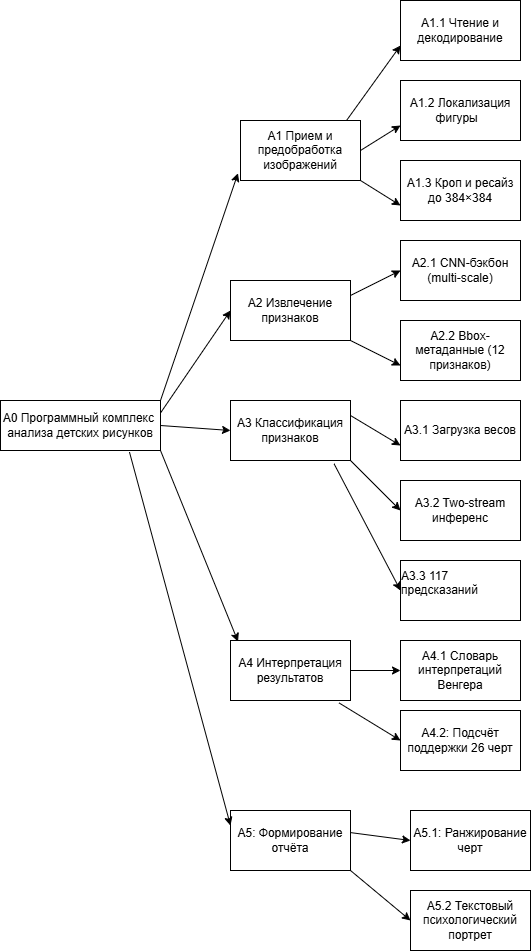
\includegraphics[width=\linewidth,height=0.55\textheight,keepaspectratio]{inc/vkr2.drawio.png}
    \caption{Функциональная декомпозиция программного комплекса анализа детских рисунков}
    \label{fig:func-decomposition}
\end{figure}

Назначение каждого модуля следующее:

\begin{itemize}
    \item A1. Приём и предобработка изображений --- принимает исходный отсканированный рисунок и подготавливает его для нейросетевой модели: чтение и декодирование файла (A1.1), локализация фигуры на основе классических методов обработки изображений (A1.2), кроп и ресайз выделенной области до размера $384 \times 384$ (A1.3);
    \item A2. Извлечение признаков --- формирует входы для нейросетевой модели: визуальные признаки кропа через свёрточный бэкбон (A2.1) и вектор bbox-метаданных из 12 геометрических характеристик (A2.2);
    \item A3. Классификация признаков --- ядро системы. Загружает веса обученной модели (A3.1), выполняет двухпотоковый инференс (A3.2) и формирует 117 предсказаний (A3.3);
    \item A4. Интерпретация результатов --- транслирует предсказания модели в психологические термины с использованием словаря, построенного на основе методики А.~Л.~Венгера (A4.1), и подсчитывает поддержку для каждой из 26 канонических черт (A4.2);
    \item A5. Формирование отчёта --- ранжирует психологические черты по числу подтверждающих признаков (A5.1) и собирает связный текстовый портрет с пояснениями (A5.2).
\end{itemize}

Каждый модуль имеет чётко определённые входы и выходы, что обеспечивает прозрачность работы системы и возможность независимой замены отдельных компонентов. На уровне реализации каждый функциональный модуль вынесен в отдельный микросервис, поверх которых построен веб-интерфейс пользователя (см.~подразделы~2.8--2.13).

\subsection{Описание датасета и его подготовка}

В работе использован датасет из 8179 отсканированных детских рисунков, полученный из образовательных учреждений Самарской области, Республики Чувашии, Московской и Вологодской областей. База изображений и разметка предоставлены Московским государственным психолого-педагогическим университетом, разметка выполнена специалистами в области детской психологии. Сопровождающая CSV-таблица содержит для каждой записи значения 117 экспертно проставленных признаков и служебные поля.

В разметке для 61 уникального кода имеется по нескольку записей с возможными расхождениями значений признаков, что объясняется независимой разметкой одного и того же рисунка несколькими экспертами. Для устранения противоречий применяется голосование большинством (majority vote) по каждому признаку независимо. После дедупликации каждому уникальному коду соответствует одна запись с консолидированной разметкой, записи без соответствующего изображения исключаются. В результате получается выборка из более 7000 примеров.

Для разбиения на обучающую, валидационную и тестовую части применяется групповое стратифицированное разбиение в пропорции 70\,/\,15\,/\,15 с использованием библиотеки iterative-stratification~\cite{iterstrat}. Стратификация выполняется по бинарным индикаторам редких классов наиболее сложных признаков. После дедупликации каждый код встречается ровно один раз, поэтому разбиение автоматически group-safe.

\subsection{Модуль предобработки изображений}

Модуль реализует локализацию фигуры человека на отсканированном листе и формирует кропированное квадратное изображение фиксированного размера и вектор из 12 геометрических метаданных. Алгоритм собран из классических операций библиотеки OpenCV~\cite{opencv} без использования предобученных нейронных моделей детекции, что обеспечивает прозрачность и воспроизводимость поведения модуля.

Конвейер обработки состоит из нескольких этапов. К исходному изображению, приведённому к одноканальному виду, применяется адаптивная бинаризация с гауссовым ядром, выбранная вместо глобального порога из-за неравномерной яркости сканов, затем медианная фильтрация и морфологическое замыкание для объединения близко расположенных штрихов одной фигуры в связную область. Далее с помощью \texttt{cv2.connectedComponentsWithStats} выделяются связные компоненты, каждая из которых проходит проверку по четырём независимым критериям: минимальная площадь, занимаемая доля листа, отношение сторон, плотность заполнения.

Из оставшихся кандидатов выбирается компонента с наибольшей площадью --- якорная, к ней присоединяются все остальные кандидаты, чьи центры масс находятся в пределах адаптивного радиуса. Результирующий ограничивающий прямоугольник расширяется на 8\,\% по каждой стороне, по нему выполняется обрезка, дополнение белым фоном до квадрата и приведение к разрешению $384 \times 384$ билинейной интерполяцией.

Помимо кропа, для каждого изображения вычисляется вектор из 12 геометрических метаданных: относительные ширина, высота, площадь и координаты центра bbox; отношение высоты к ширине; четыре бинарных индикатора касания краёв листа; нормализованное расстояние от центра bbox до ближайшего угла; индикатор источника детекции. Эти метаданные используются как второй вход нейронной сети (см.~подраздел~2.4) и сохраняют информацию о размере и положении фигуры на исходном листе, утрачиваемую после кропа.

\subsection{Архитектура нейросетевой модели}

Для классификации 117 признаков спроектирована двухпотоковая свёрточная нейронная сеть, обучаемая полностью с нуля на целевой выборке детских рисунков. Общая схема архитектуры приведена в приложении на рисунке~\ref{fig:drawingnet-arch-appendix}.

Выбор обучения с нуля вместо transfer learning с предобученным бэкбоном (например, ResNet-50) мотивирован существенным отличием статистики детских карандашных рисунков от естественных фотоизображений ImageNet. ImageNet-предобучение оптимизирует свёрточные ядра под детектирование цветных текстур и градиентов яркости, в то время как карандашный рисунок представляет собой набор тёмных линий на однородном светлом фоне. В предварительных экспериментах модели на основе предобученного ResNet-50/152 не давали статистически значимого выигрыша по F1-мере над моделью, обученной с нуля, при существенно большем числе параметров (около 60 млн против 5,5 млн у разработанной модели).

Первый поток обрабатывает кропированное изображение размером $320 \times 320$ пикселей. Уменьшение разрешения с $384$ до $320$ выполнено для сокращения объёма вычислений на инференсе без существенной потери качества (потеря F1 в предварительных экспериментах --- около 0,003). Сеть состоит из пяти этапов:

\begin{itemize}
    \item Stem --- первый свёрточный слой с ядром $7 \times 7$, BatchNorm~\cite{batchnorm}, ReLU и max-pool $3 \times 3$ со страйдом 2. Большое начальное ядро мотивировано особенностью детских рисунков: типичные карандашные штрихи длинные, и одно ядро $7 \times 7$ захватывает целые сегменты, в отличие от стандартных ядер $3 \times 3$ современных backbone'ов;
    \item Stage~2 (64 канала) --- два residual-блока с последующим max-pool;
    \item Stage~3 (128 каналов) --- два residual-блока с последующим max-pool;
    \item Stage~4 (256 каналов) --- два residual-блока с последующим max-pool, выход используется как первый источник многомасштабных признаков;
    \item Stage~5 (384 канала) --- один residual-блок, выход используется как второй источник многомасштабных признаков.
\end{itemize}

Каждый residual-блок реализует стандартную схему с двумя свёртками $3 \times 3$, BatchNorm и ReLU и пропускающим (skip) соединением. При несовпадении числа каналов или страйда в skip-соединение добавляется проекционная свёртка $1 \times 1$. Использование residual-связей обеспечивает устойчивое распространение градиентов в глубокой сети и облегчает оптимизацию~\cite{resnet}.

С целью повышения детализации признакового представления используется конкатенация выходов четвёртого и пятого этапов, пропущенных через адаптивный усредняющий пулинг до размера $1 \times 1$:
\begin{equation}
\mathbf{f}_{img} = \left[\, \text{pool}(\text{stage}_4(x))\ ;\ \text{pool}(\text{stage}_5(x)) \,\right] \in \mathbb{R}^{640}
\end{equation}

Применение конкатенации признаков с двух уровней обусловлено следующими соображениями. Признаки stage~4 (256 каналов) содержат среднеуровневые геометрические паттерны (формы, очертания, локальные особенности), полезные для распознавания мелких деталей рисунка (форма глаз, наличие пуговиц, штриховка). Признаки stage~5 (384 канала) содержат высокоуровневые семантические признаки, релевантные для общих характеристик (поза фигуры, ракурс, размер). Совместное использование обоих уровней даёт богатое признаковое представление, способное обслуживать как мелкозернистые, так и крупнозернистые задачи распознавания.

Второй поток обрабатывает 12-мерный вектор геометрических метаданных, выработанных модулем предобработки. Перед подачей в сеть метаданные нормируются по среднему и стандартному отклонению, вычисленным на обучающей выборке. Преобразование выполняет двухслойный MLP с активациями ReLU и одним слоем дропаута~\cite{dropout}:
\begin{equation}
\mathbf{f}_{bbox} = \text{MLP}(\mathbf{x}_{bbox}) \in \mathbb{R}^{64}
\end{equation}

Необходимость второго потока обусловлена тем, что после кропа и ресайза фигуры к фиксированному размеру в визуальном представлении теряется информация о её абсолютном размере и положении на исходном листе. Между тем эта информация существенна для ряда признаков рисуночного теста: <<размер рисунка>> определяется отношением площади фигуры к площади листа, <<расположение>> и <<смещение>> --- координатами центра фигуры на странице, признак <<обрезано>> --- касанием bbox-фигуры краёв листа.

Векторы признаков от двух потоков конкатенируются и пропускаются через одну из двух параллельных проекционных голов. Признаки, для которых ожидается повышенная сложность распознавания, направляются через выделенную проекцию; остальные --- через общую проекцию. Такое разделение --- разновидность многозадачного обучения с группировкой задач~\cite{multitask-survey} --- уменьшает конкуренцию градиентов между задачами разной сложности и обеспечивает более устойчивое обучение признаков с малым числом примеров. Каждая проекция сужает признаковое пространство до 256 нейронов с дропаутом 0,3.

Финальный слой состоит из 117 параллельных классификационных голов: каждая голова --- один линейный слой, отображающий 256-мерный признак в логиты соответствующего числа классов (2 для бинарного признака, $K$ для категориального с $K$ классами). Все 117 голов организованы в виде \texttt{nn.ModuleDict}, что обеспечивает прозрачную адресацию к голове по имени критерия и упрощает сохранение и загрузку модели.

Общее число параметров модели составляет около 5,5~миллионов, размер сохранённого чекпоинта --- около 22~МБ. Инициализация всех свёрточных и линейных слоёв выполнена методом Кайминга~\cite{kaiming-init}, что соответствует выбранной активации ReLU и обеспечивает корректное масштабирование начальных активаций по слоям. На рисунке~\ref{src:src3} представлен фрагмент реализации определения архитектуры модели и процедуры обучения.

\begin{figure}
    \lstinputlisting[language=Python]{inc/code2.py}
    \caption{Фрагмент кода реализации обучения}
    \label{src:src3}
\end{figure}

\subsection{Функции потерь и стратегия обучения}

Для бинарного признака используется взвешенная перекрёстная энтропия с весами классов $\alpha = (1.0,\ \min(\sqrt{N_-/N_+},\ 10))$, где $N_\pm$ --- количества отрицательных и положительных примеров. Корень из отношения и ограничение значением 10 защищают градиент от взрыва при экстремальном дисбалансе. В качестве альтернативы рассматривалась фокальная функция потерь~\cite{focal-loss}, однако сочетание корневого взвешивания и WeightedRandomSampler даёт сопоставимое поведение при меньшем числе гиперпараметров для подбора.

Для категориального признака используется взвешенная перекрёстная энтропия с label smoothing $0.05$ и весами $\alpha_i = \min(\sqrt{N_{max}/N_i},\ 10)$. Совокупная функция потерь --- среднее по 117 признакам:
\begin{equation}
\mathcal{L} = \frac{1}{117} \sum_{i=1}^{117} \mathcal{L}_i(\mathbf{f}_{proj},\ y_i)
\end{equation}

Дополнительно применяется WeightedRandomSampler: каждому примеру обучающей выборки присваивается вес, повышенный относительно базового для тех примеров, которые имеют положительные метки редких классов. Веса ограничены диапазоном $[1, 2.5]$, сэмплирование выполняется с возвращением. На рисунке~\ref{src:src4} приведён фрагмент реализации цикла обучения с вычислением функций потерь и обновлением параметров модели.

\begin{figure}
    \lstinputlisting[language=Python]{inc/code3.py}
    \caption{Фрагмент кода реализации цикла обучения}
    \label{src:src4}
\end{figure}

К каждому изображению применяется набор аугментаций: random affine ($\pm6^\circ$, сдвиг до 5\,\%, масштаб 90--110\,\%), random crop из увеличенного на 32~пикселя изображения до $320\times320$, color jitter (яркость и контраст до 15\,\%), random erasing с вероятностью 0,2. Намеренно не используется горизонтальное отражение, поскольку ряд признаков содержит указание на правую и левую стороны.

Оптимизатор --- AdamW~\cite{adamw,adam} с базовой скоростью обучения $10^{-4}$, weight decay $5 \cdot 10^{-4}$, обрезкой нормы градиента до 1,0. Размер пакета --- 32. Расписание LR --- косинусное затухание с разогревом в течение трёх эпох~\cite{cosine-schedule}. Смешанная точность намеренно отключена в пользу одинарной (fp32): при обучении с нуля и сильных весовых коэффициентах функции потерь начальные градиенты могут принимать большие значения, и в режиме fp16 это иногда приводит к численным переполнениям. Полное число эпох --- 50 с ранней остановкой по отсутствию улучшения F1 на валидации в течение 8 эпох с минимумом в 25 эпох.

\subsection{Словарь интерпретаций признаков}

Связь между техническими признаками рисунка и психологическими чертами реализована через JSON-словарь \texttt{criteria\_interpretations.json} объёмом около 60~КБ. Структура словаря: раздел \texttt{traits} --- 26 канонических черт с текстовыми описаниями; раздел \texttt{criteria} --- 117 признаков с указанием типа, набора связанных черт; раздел \texttt{meta} --- сведения о версии и источниках. Содержательная составляющая построена на основе книги А.~Л.~Венгера~\cite{venger}.

Один признак может быть индикатором нескольких черт, а одна черта обычно поддерживается набором различных признаков. При использовании словаря в составе генератора портрета каждой черте сопоставляется счётчик поддержки, равный количеству предсказанных моделью признаков, ассоциированных с ней. Это позволяет ранжировать черты в итоговом тексте по степени их выраженности. В таблице~\ref{traits-list} приведена часть канонических черт.

\begin{table}
    \caption{Часть канонических психологических черт}
    \fontsize{12pt}{14pt}\selectfont
    \begin{tabular}{|p{60mm}|p{90mm}|}\hline
        \textbf{Черта} & \textbf{Краткое пояснение} \\ \hline
        Тревожность личностная           & Устойчивая склонность к беспокойству, сниженная самооценка \\ \hline
        Состояние тревоги                & Ситуативная тревога, проявленная в момент рисования \\ \hline
        Демонстративность                & Стремление быть в центре внимания, экспансивное поведение \\ \hline
        Агрессивность                    & Склонность к враждебному, конкурентному поведению \\ \hline
    \end{tabular}
    \label{traits-list}
\end{table}

\subsection{Генератор текстового психологического портрета}

Модуль принимает на вход словарь предсказаний модели $\{c_i \mapsto v_i\}_{i=1}^{117}$ и словарь интерпретаций. Для каждого признака с положительным предсказанием ($v_i \neq 0,\ v_i \neq \text{пусто}$) извлекается соответствующий список черт, и для каждой черты $t$ инкрементируется счётчик поддержки:
\begin{equation}
S(t) = \sum_{i=1}^{117} \mathbb{1}\big[\, t \in \text{traits}(c_i, v_i) \,\big]
\end{equation}
Параллельно для каждой черты накапливается список свидетельств --- пар <<признак, значение>>, давших вклад в её поддержку.

Финальный текст портрета содержит заголовок и краткое пояснение, перечень из 7 наиболее устойчиво проявленных черт с порогом поддержки не менее 2 признаков --- для каждой приводится описание и до 4 подтверждающих свидетельств, --- раздел менее устойчивых тенденций с поддержкой 1 признака и итоговое замечание о вероятностном характере выводов. Объём типового портрета --- 25--40 строк. На рисунке~\ref{src:src5} представлен фрагмент кода, реализующий логику формирования психологического портрета на основе предсказаний модели и словаря интерпретаций.

\begin{figure}
    \lstinputlisting[language=Python]{inc/code4.py}
    \caption{Фрагмент кода для генерации психологического портрета}
    \label{src:src5}
\end{figure}

\subsection{Микросервисная архитектура веб-сервиса}

Программный комплекс реализован в виде микросервисного веб-приложения, архитектура которого представлена на рисунке~\ref{fig:veb-arch}. Система разделена на три логических контура, объединённых единым API-шлюзом.

\begin{figure}
    \centering
    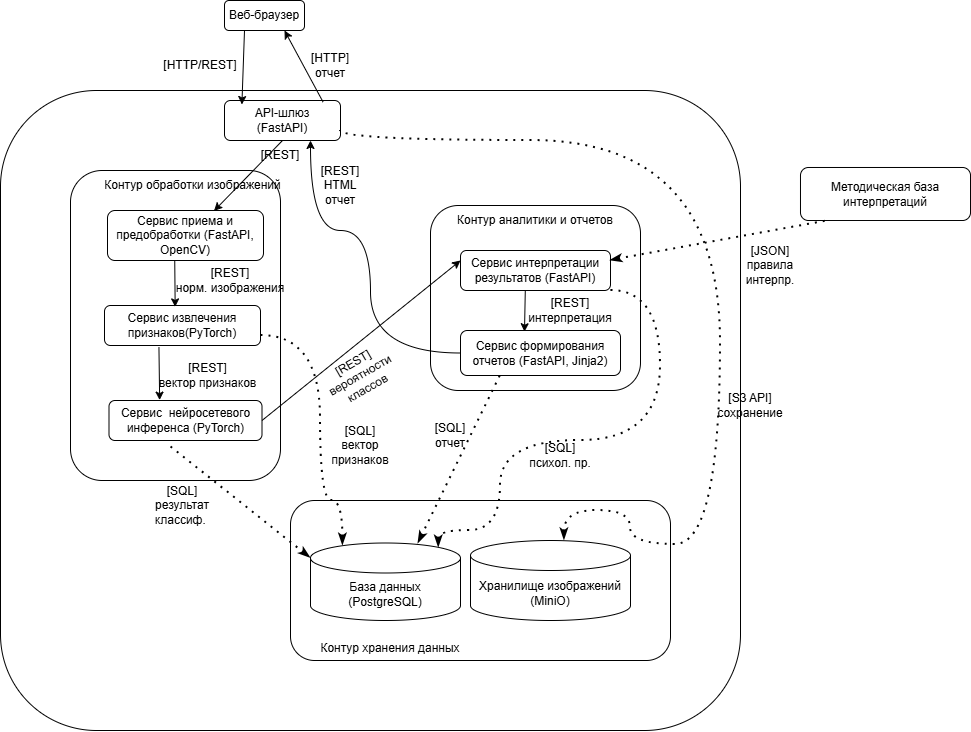
\includegraphics[width=\linewidth,height=0.6\textheight,keepaspectratio]{inc/veb-arch.png}
    \caption{Архитектура веб-сервиса: микросервисы, протоколы взаимодействия и контуры хранения данных}
    \label{fig:veb-arch}
\end{figure}

API-шлюз (FastAPI~\cite{fastapi}) --- единственная точка входа для внешнего пользователя. Принимает HTTP/REST-запросы от веб-браузера, оркестрирует последовательные вызовы к внутренним сервисам и возвращает итоговый HTML-отчёт. Шлюз также отвечает за сохранение изображений в объектное хранилище MinIO~\cite{minio} (S3 API) и метаданных анализа в реляционную базу PostgreSQL~\cite{postgres}.

Контур обработки изображений включает три сервиса, образующих последовательный конвейер:

\begin{enumerate}
    \item сервис приёма и предобработки (FastAPI~\cite{fastapi}, OpenCV~\cite{opencv}) --- принимает исходное изображение, выполняет локализацию фигуры и возвращает нормализованное изображение и координаты bbox;
    \item сервис извлечения признаков (FastAPI~\cite{fastapi}) --- вычисляет 12-мерный вектор геометрических метаданных на основе координат bbox;
    \item сервис нейросетевого инференса (PyTorch~\cite{pytorch}) --- загружает обученную модель и выполняет классификацию: принимает изображение и вектор признаков, возвращает вероятности 117~классов.
\end{enumerate}

Между сервисами контура данные передаются по REST: нормализованное изображение и вектор признаков последовательно проходят через конвейер. Результат классификации в виде вероятностей классов передаётся в следующий контур.

Контур аналитики и отчётов включает два сервиса:

\begin{enumerate}
    \item сервис интерпретации результатов (FastAPI~\cite{fastapi}) --- принимает вектор вероятностей классов и транслирует его в психологические черты с использованием методической базы интерпретаций (JSON-словарь, построенный по методике А.~Л.~Венгера~\cite{venger});
    \item сервис формирования отчётов (FastAPI~\cite{fastapi}) --- принимает интерпретацию и формирует HTML-документ психологического портрета, который возвращается API-шлюзу.
\end{enumerate}

Контур хранения данных обеспечивает персистентность:

\begin{itemize}
    \item база данных (PostgreSQL~\cite{postgres}) --- хранит метаданные анализов, предсказания модели, поддержку черт и сгенерированные портреты;
    \item хранилище изображений (MinIO~\cite{minio}) --- хранит исходные сканы рисунков и результаты предобработки через S3-совместимый интерфейс.
\end{itemize}

Все внутренние сервисы взаимодействуют по протоколу REST через локальную Docker-сеть~\cite{docker}. Внешний доступ открыт только для API-шлюза (порт 8000); остальные сервисы изолированы от внешних запросов, что снижает поверхность атаки.

Такая архитектура обеспечивает независимое масштабирование отдельных компонентов --- при увеличении нагрузки можно горизонтально масштабировать только сервис инференса, --- технологическую независимость сервисов, отказоустойчивость, при которой сбой одного сервиса не приводит к падению системы, и возможность замены модели без затрагивания остальных компонентов.

Состав сервисов и их порты приведены в таблице~\ref{services-list}.

\begin{table}
    \caption{Состав микросервисов программного комплекса}
    \fontsize{12pt}{14pt}\selectfont
    \begin{tabular}{|p{30mm}|p{15mm}|p{99mm}|}\hline
        \textbf{Сервис} & \textbf{Порт} & \textbf{Назначение} \\ \hline
        api-gateway      & 8000  & Веб-интерфейс, оркестрация цепочки, сохранение результата в БД и MinIO \\ \hline
        preprocessing    & 8001  & Локализация фигуры (OpenCV~\cite{opencv} + YOLO-резерв~\cite{yolov8}), кроп и ресайз до $384 \times 384$ \\ \hline
        features         & 8002  & Вычисление 12 геометрических bbox-признаков \\ \hline
        inference        & 8003  & Нейросетевой инференс: $\text{(image, bbox)} \mapsto 117$ предсказаний \\ \hline
        interpretation   & 8004  & Маппинг 117 предсказаний $\rightarrow$ 26 психологических черт \\ \hline
        report           & 8005  & Рендер HTML-портрета по шаблону Jinja2 \\ \hline
    \end{tabular}
    \label{services-list}
\end{table}

\subsection{Технологический стек}

В качестве основного языка разработки выбран Python~3.11 ввиду того, что обученная нейросетевая модель и алгоритмы предобработки изображений уже реализованы на этом языке. Для построения REST-сервисов используется фреймворк FastAPI~\cite{fastapi} с автоматической генерацией OpenAPI-схемы и валидацией входных данных через Pydantic. ASGI-сервер --- Uvicorn~\cite{uvicorn}.

Сервис инференса использует библиотеку PyTorch~\cite{pytorch} для загрузки и выполнения нейросетевой модели, сервис предобработки --- библиотеки OpenCV~\cite{opencv} (адаптивная бинаризация, морфология, выделение связных компонент) и Ultralytics (резервный YOLOv8-детектор~\cite{yolov8}). Для межсервисного взаимодействия по HTTP используется асинхронный клиент httpx, шаблонизатор для HTML-портретов и веб-интерфейса --- Jinja2.

Сервис \texttt{api-gateway} взаимодействует с внешними системами хранения через стандартизированные клиенты: \texttt{psycopg} (PostgreSQL) и \texttt{minio} (MinIO S3-совместимое объектное хранилище). Все библиотечные зависимости каждого сервиса вынесены в \texttt{requirements.txt} и устанавливаются изолированно при сборке образа.

\subsection{Описание сервисов}

api-gateway --- единственная точка входа для пользователя. Предоставляет HTML-форму загрузки рисунка на главной странице, страницу истории анализов и страницу повторного просмотра сохранённого портрета по его идентификатору. При получении нового запроса сервис генерирует UUID анализа, последовательно вызывает остальные сервисы, сохраняет промежуточные результаты в MinIO, а финальный результат --- в PostgreSQL. HTML-шаблоны (форма загрузки, история, страница ошибки) выполнены на Jinja2.

preprocessing --- реализует алгоритм локализации фигуры из подраздела~2.3. На вход поступает multipart-файл изображения, на выход --- base64-кодированный кроп размером $384 \times 384$, координаты bbox на исходном листе, размеры исходного изображения и индикатор источника детекции. Если основной OpenCV-алгоритм не обнаруживает достаточно крупной связной области, выполняется резервная детекция через YOLOv8 --- готовый детектор людей используется в роли подстраховки, что повышает робастность системы к редким сложным случаям сканирования.

features --- лёгкий вычислительный сервис, принимающий координаты bbox и размеры исходного листа и возвращающий вектор из 12 геометрических признаков, описанных в подразделе~2.3. Сервис не содержит ML-зависимостей, выполняется в считанные миллисекунды и легко горизонтально масштабируется.

inference --- ядро системы. При запуске контейнера загружает веса обученной модели, словари label encoders, а также маски \texttt{target/nontarget}, восстановленные из вспомогательного pickle-файла \texttt{encoders.pkl}. На вход принимает изображение и 12-мерный вектор bbox-фичей; на выход выдаёт словарь 117 предсказаний и сопутствующих confidences (значения softmax по предсказанному классу). Сервис не требует GPU --- инференс выполняется на CPU за порядка 0,2~секунды на одно изображение.

interpretation --- применяет словарь \texttt{criteria\_interpretations.json} к 117 предсказаниям, формирует словарь поддержки 26 черт и список свидетельств (см.~подраздел~2.7). Логика модуля не содержит обучаемых параметров и реализована на чистом Python.

report --- финальный шаг конвейера. Принимает словарь черт, список свидетельств и (опционально) ссылки на изображения в MinIO, формирует HTML-документ психологического портрета по шаблону Jinja2 с применением CSS-стилей. Сгенерированный HTML возвращается обратно \texttt{api-gateway}, который сохраняет его в PostgreSQL и отдаёт пользователю.

\subsection{Хранение данных}

Хранение данных распределено между двумя внешними системами в соответствии с типами хранимых данных.

Реляционная СУБД PostgreSQL~\cite{postgres} версии 16 хранит метаданные анализов: уникальный идентификатор, временную метку, оригинальное имя файла, ключи в объектном хранилище, источник детекции, словарь 117 предсказаний, словарь поддержки 26 черт и сгенерированный HTML-портрет. Структура одной таблицы \texttt{analyses} приведена в приложении. На полях временной метки и источника детекции созданы B-tree индексы для ускорения выборки в истории анализов. Хранение предсказаний и поддержки в виде JSONB позволяет гибко расширять формат без миграций схемы.

Объектное хранилище MinIO~\cite{minio} хранит бинарные файлы --- исходные сканы рисунков и кропы, выработанные модулем предобработки. Ключи объектов имеют структуру \texttt{drawings/\{analysis\_id\}/\{original|cropped\}.png}, что обеспечивает однозначное соответствие между записью в PostgreSQL и связанными с ней файлами. MinIO выбран в качестве замены прямого хранения файлов в файловой системе по нескольким причинам: совместимый с Amazon S3 интерфейс упрощает миграцию в облако; встроенная веб-консоль обеспечивает прямой доступ к содержимому для администратора; разделение бинарных файлов и метаданных согласуется с микросервисной идеологией.

Такое разделение обеспечивает выполнение основного принципа проектирования: метаданные хранятся в РСУБД, где они индексируются и связываются по отношениям, а бинарные файлы --- в объектном хранилище, где их объём не влияет на производительность РСУБД.

\subsection{Контейнеризация и развёртывание}

Все сервисы и системы хранения упакованы в Docker-контейнеры~\cite{docker}; для запуска используется единый файл \texttt{docker-compose.yml}, описывающий граф зависимостей между сервисами, переменные окружения, тома для постоянного хранения данных и проброс портов. Сборка каждого сервиса выполняется из собственного \texttt{Dockerfile} в каталоге \texttt{services/<service-name>/}; общие данные (веса модели, словари) монтируются как read-only том из директории \texttt{shared/data/} в путь \texttt{/data} внутри контейнеров.

В составе \texttt{docker-compose.yml} выделены три логических контура: контур обработки изображений (preprocessing, features, inference), контур аналитики и отчётов (interpretation, report), контур хранения (postgres, minio). Шлюз \texttt{api-gateway} оркестрирует обращения ко всем трём контурам и предоставляет единый внешний интерфейс на порту 8000. Дополнительно описан профиль \texttt{tools}, в котором одноразово запускается утилита \texttt{encoders-builder}, собирающая из исходных CSV-таблиц консолидированный pickle-файл с label encoders для сервиса инференса.

Все сервисы конфигурируются через переменные окружения, перечисленные в файле \texttt{.env}, что позволяет менять конфигурацию (имена базы, пароли, URL внутренних сервисов) без пересборки образов. Для запуска полного стека достаточно одной команды \texttt{docker compose up}, что упрощает развёртывание на новом сервере или локальной машине разработчика.

\subsection{Поток данных при анализе одного рисунка}

При загрузке нового рисунка через веб-интерфейс выполняется следующая последовательность обращений между сервисами:

\begin{enumerate}
    \item \texttt{api-gateway} принимает HTTP POST с файлом изображения, генерирует идентификатор анализа (UUID), сохраняет оригинал в MinIO по ключу \texttt{drawings/\{id\}/original.png};
    \item обращение к \texttt{preprocessing}\,/crop --- модуль возвращает кроп в base64, координаты bbox, размеры исходного изображения и источник детекции;
    \item полученный кроп сохраняется в MinIO по ключу \texttt{drawings/\{id\}/cropped.png};
    \item обращение к \texttt{features}\,/compute с координатами bbox и размерами оригинала --- модуль возвращает вектор из 12 геометрических признаков;
    \item обращение к \texttt{inference}\,/predict с изображением и вектором bbox-фичей --- модуль возвращает 117 предсказаний и их confidences;
    \item обращение к \texttt{interpretation}\,/derive с 117 предсказаниями --- модуль возвращает поддержку 26 черт и список свидетельств;
    \item обращение к \texttt{report}\,/render с данными о чертах и свидетельствами --- модуль возвращает HTML-документ психологического портрета;
    \item \texttt{api-gateway} сохраняет в Postgres метаданные анализа (идентификатор, ключи в MinIO, предсказания, поддержку черт, HTML-портрет) и возвращает HTML пользователю.
\end{enumerate}

Все обращения между сервисами выполняются по локальной docker-сети с использованием доменных имён сервисов (например, \texttt{http://inference:8003/predict}), не выходят за пределы хоста и не предполагают аутентификации. Пользовательский интерфейс взаимодействует только с \texttt{api-gateway} через порт 8000.

Сохранённый результат доступен в дальнейшем через раздел истории анализов и может быть открыт повторно по идентификатору без выполнения цепочки заново --- сохранённый HTML-портрет извлекается из PostgreSQL и отдаётся пользователю без обращения к остальным сервисам. Это обеспечивает быстрый просмотр уже выполненных анализов и снижает нагрузку на сервис инференса.
    
    \section{ЭКСПЕРИМЕНТАЛЬНОЕ ИССЛЕДОВАНИЕ}

\subsection{Условия проведения экспериментов}

Все эксперименты проводились в облачной среде Google Colab Notebooks с использованием графического ускорителя NVIDIA Tesla T4, 16~ГБ видеопамяти. Программное окружение: Python~3.10, PyTorch~2.x с поддержкой CUDA, библиотеки torchvision, opencv-python, pandas, scikit-learn, iterative-stratification.

Размер пакета при обучении --- 32 примера, размер изображения --- $320 \times 320$ пикселей, число эпох --- 50 с ранней остановкой. Время обучения одной эпохи составляет около 60 секунд, полный цикл обучения занимает около 30--50 минут в зависимости от срабатывания ранней остановки.

Воспроизводимость обеспечивается фиксированным значением \texttt{random\_state} = 42 для всех источников случайности: разбиения выборки, инициализации весов сети, перемешивания данных и взвешенного сэмплирования.

\subsection{Метрики качества}

Для оценки качества модели применяются три варианта F1-меры~\cite{f1-score}:

\begin{itemize}
    \item F1\textsubscript{micro} --- F1, вычисленная по агрегированной матрице ошибок с одинаковым весом каждого предсказания. В целом, можно сказать близка к accuracy и отражает общую долю правильных предсказаний;
    \item F1\textsubscript{weighted} --- среднее F1 по классам с весами, пропорциональными количеству примеров каждого класса в выборке. Учитывает редкость классов, не штрафуя избыточно за их пропуск;
    \item F1\textsubscript{macro} --- среднее значение F1 по классам каждого признака с равными весами для всех классов независимо от их частоты. Чувствительна к качеству модели на минорных классах.
\end{itemize}

Формально метрики определяются следующим образом. Для каждого класса $c$ определяются количества истинно положительных (TP$_c$), ложно положительных (FP$_c$) и ложно отрицательных (FN$_c$) предсказаний. Точность (precision) и полнота (recall) для класса $c$:  

\begin{equation}
P_c = \frac{\text{TP}_c}{\text{TP}_c + \text{FP}_c}, \quad R_c = \frac{\text{TP}_c}{\text{TP}_c + \text{FN}_c}
\end{equation}

F1\textsubscript{micro} агрегирует TP, FP, FN по всем классам перед вычислением:
\begin{equation}
\text{F1}_{\text{micro}} = \frac{2 \sum_c \text{TP}_c}{2 \sum_c \text{TP}_c + \sum_c \text{FP}_c + \sum_c \text{FN}_c}
\end{equation}

F1\textsubscript{macro} вычисляет F1 для каждого класса отдельно и усредняет с равным весом:
\begin{equation}
\text{F1}_{\text{macro}} = \frac{1}{C} \sum_{c=1}^{C} \frac{2\, P_c \cdot R_c}{P_c + R_c}
\end{equation}

F1\textsubscript{weighted} усредняет F1 по классам с весами, пропорциональными числу примеров $n_c$ каждого класса:
\begin{equation}
\text{F1}_{\text{weighted}} = \frac{\sum_{c=1}^{C} n_c \cdot \text{F1}_c}{\sum_{c=1}^{C} n_c}
\end{equation}

Каждая из трёх метрик имеет своё практическое значение. F1\textsubscript{micro} и F1\textsubscript{weighted} отражают качество системы на типичных рисунках --- то, как часто модель будет давать корректное предсказание для произвольно выбранного образца. F1\textsubscript{macro} показывает, насколько хорошо модель справляется со всеми классами одновременно, в том числе с теми, которые встречаются редко. В работе все три метрики приводятся параллельно, без выбора одной из них в качестве главной.

В качестве итоговых показателей по всем 117 признакам используются средние значения F1 каждого вида, рассчитанные как среднее арифметическое по 117 признакам.

\subsection{Результаты на тестовой выборке}

Результаты, полученные разработанной моделью на тестовой выборке, которая составляет около 1000 рисунков, приведены в таблице~\ref{main-results}.

\begin{table}
    \caption{Метрики качества на тестовой выборке}
    \fontsize{12pt}{18pt}\selectfont
    \begin{tabular}{|l|c|}\hline
        \textbf{Метрика}                      & \textbf{Значение}  \\ \hline
        F1\textsubscript{micro}               & 0,901              \\ \hline
        F1\textsubscript{weighted}            & 0,875              \\ \hline
        F1\textsubscript{macro}               & 0,521              \\ \hline
    \end{tabular}
    \label{main-results}
\end{table}

Значение F1\textsubscript{micro} = 0,901 означает, что модель корректно классифицирует около 90\,\% всех предсказаний по 117 признакам в совокупности. Близкое к нему значение F1\textsubscript{weighted} = 0,875 подтверждает устойчивость качества при учёте различной частоты классов. Отличия между двумя метриками невелики, что указывает на отсутствие систематического перекоса в сторону какой-либо группы классов.

Заметно более низкое значение F1\textsubscript{macro} = 0,521 объясняется особенностями выборки и формулы метрики. F1\textsubscript{macro} штрафует модель за каждый минорный класс, который она не научилась распознавать, причём с равным весом независимо от размера класса. В рассматриваемом датасете 10 из 117 признаков имеют менее десяти положительных примеров в обучающей выборке. Для таких признаков модель в большинстве случаев предсказывает мажоритарный класс, что обеспечивает высокую общую точность, но низкую F1-меру по минорному классу. Эти 10 признаков существенно опускают среднее значение F1\textsubscript{macro}, не влияя при этом на F1\textsubscript{micro} и F1\textsubscript{weighted}.

При этом по ряду конкретных признаков разработанная модель превосходит результаты предыдущей базовой версии ResNet-152. В таблице~\ref{tab:improved-criteria} приведены признаки, для которых удалось улучшить метрику F1\textsubscript{macro}.

\begin{table}
    \caption{Признаки с улучшением F1\textsubscript{macro} относительно базовой модели}
    \fontsize{12pt}{18pt}\selectfont
    \begin{tabular}{|l|c|c|c|}\hline
        \textbf{Признак} & \textbf{Базовая} & \textbf{Разработанная} & \textbf{Прирост} \\ \hline
        размер глаз | большие    & 0,832 & 1,000 & +0,168 \\ \hline
        форма глаз | большие     & 0,856 & 1,000 & +0,144 \\ \hline
        ступни | отсутствуют     & 0,500 & 0,643 & +0,143 \\ \hline
    \end{tabular}
    \label{tab:improved-criteria}
\end{table}

Улучшение по данным признакам объясняется тем, что разработанная модель обучена с нуля на целевом домене карандашных рисунков без использования ImageNet-предобучения. Свёрточные фильтры, настроенные непосредственно на штриховые изображения, более чувствительны к тонким различиям в пропорциях элементов (размер и форма глаз) и наличию/отсутствию мелких деталей (ступни).

\subsection{Анализ распределения метрик по признакам}

Распределение значений F1\textsubscript{weighted} по 117 признакам приведено на рисунке~\ref{fig:f1-distribution}.

\begin{figure}[h]
    \centering
    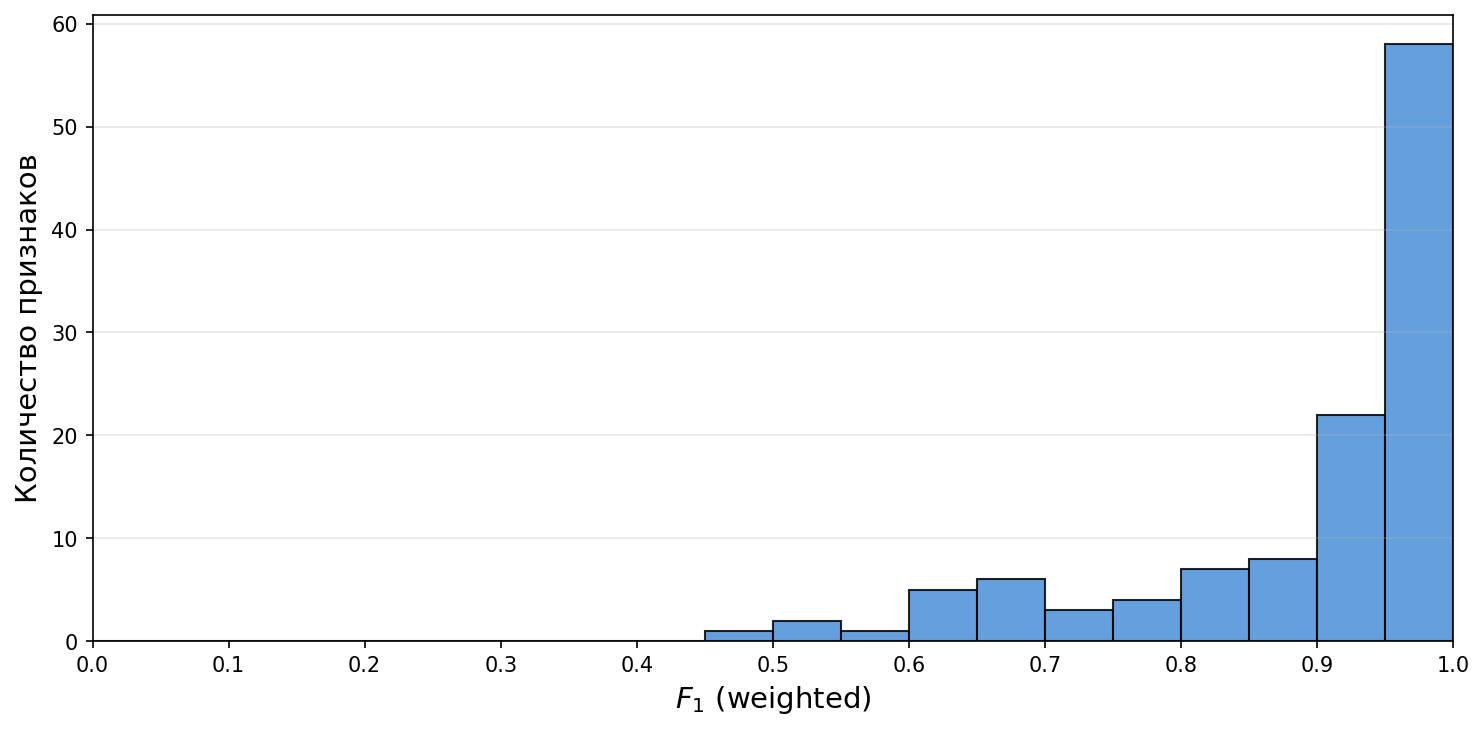
\includegraphics[width=0.85\linewidth]{inc/f1-distribution.png}
    \caption{Распределение F1\textsubscript{weighted} по 117 признакам}
    \label{fig:f1-distribution}
\end{figure}

Подавляющее большинство признаков имеет значение F1\textsubscript{weighted} в диапазоне 0,85--0,99, что подтверждает однородно высокое качество модели по совокупности задач.

Среди 117 признаков особо выделяются 10 признаков с экстремально малым числом положительных примеров (менее 10 в обучающей выборке). Для них объём данных принципиально не позволяет обучить классификатор, надёжно распознающий минорный класс: модель в большинстве случаев предсказывает мажоритарный класс, что обеспечивает высокое значение F1\textsubscript{weighted} (близкое к 1) и низкое значение F1\textsubscript{macro} (около 0,5). Эти признаки оказывают значительное влияние на среднее значение F1\textsubscript{macro} по всей выборке, но практически не влияют на F1\textsubscript{micro} и F1\textsubscript{weighted}.

В целом распределение метрик показывает, что модель успешно справляется с задачей классификации признаков рисунка для типичных рисунков. Снижение F1\textsubscript{macro} обусловлено редкими признаками, для которых при имеющемся объёме обучающих данных надёжная классификация минорного класса принципиально невозможна.

\subsection{Демонстрация работы программного комплекса}

Для демонстрации работы веб-сервиса загрузим рисунок из тестовой выборки через пользовательский интерфейс и проследим результат на каждом этапе конвейера.

На рисунке~\ref{fig:demo-header} представлена верхняя часть страницы результата: заголовок, метаинформация об анализе (число активных предсказаний, уникальный идентификатор), а также сравнение исходного отсканированного листа и результата предобработки --- кропированной и нормализованной фигуры.

\begin{figure}[h]
    \centering
    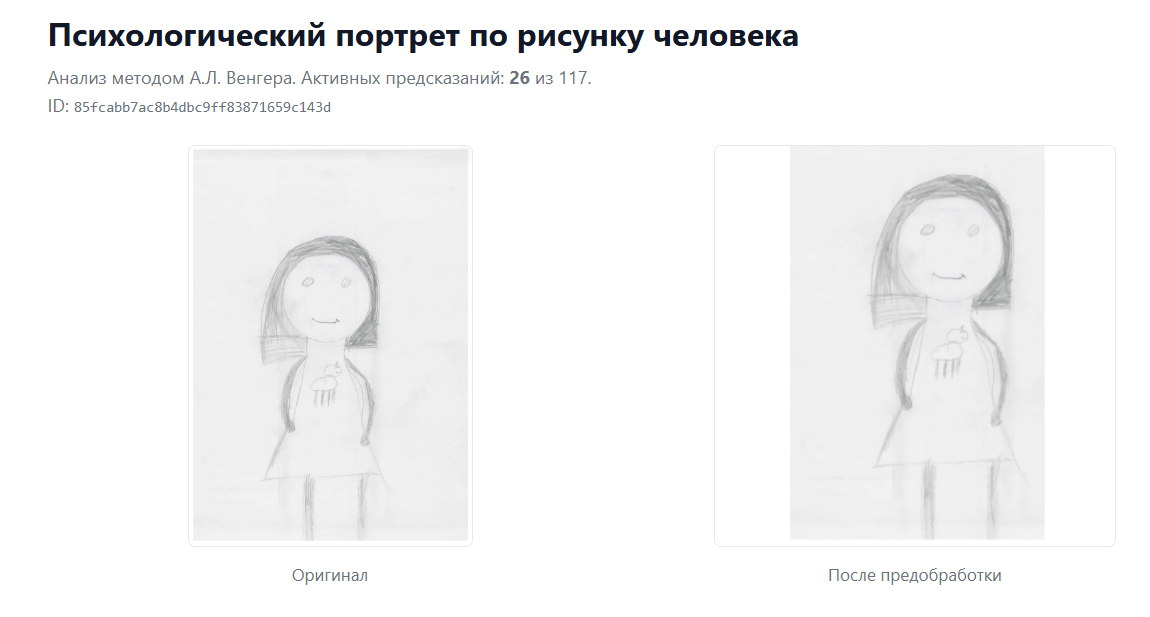
\includegraphics[width=0.8\linewidth]{inc/s1.png}
    \caption{Веб-интерфейс результата анализа: заголовок, метаданные и сравнение исходного изображения с результатом предобработки}
    \label{fig:demo-header}
\end{figure}

После прохождения изображения через нейросетевую модель 117 предсказаний транслируются через словарь интерпретаций в психологические черты. На рисунке~\ref{fig:demo-traits} показан раздел <<Ключевые особенности>> --- черты с поддержкой не менее двух признаков, ранжированные по степени выраженности. Для каждой черты указаны описание и список подтверждающих свидетельств.

\begin{figure}[h]
    \centering
    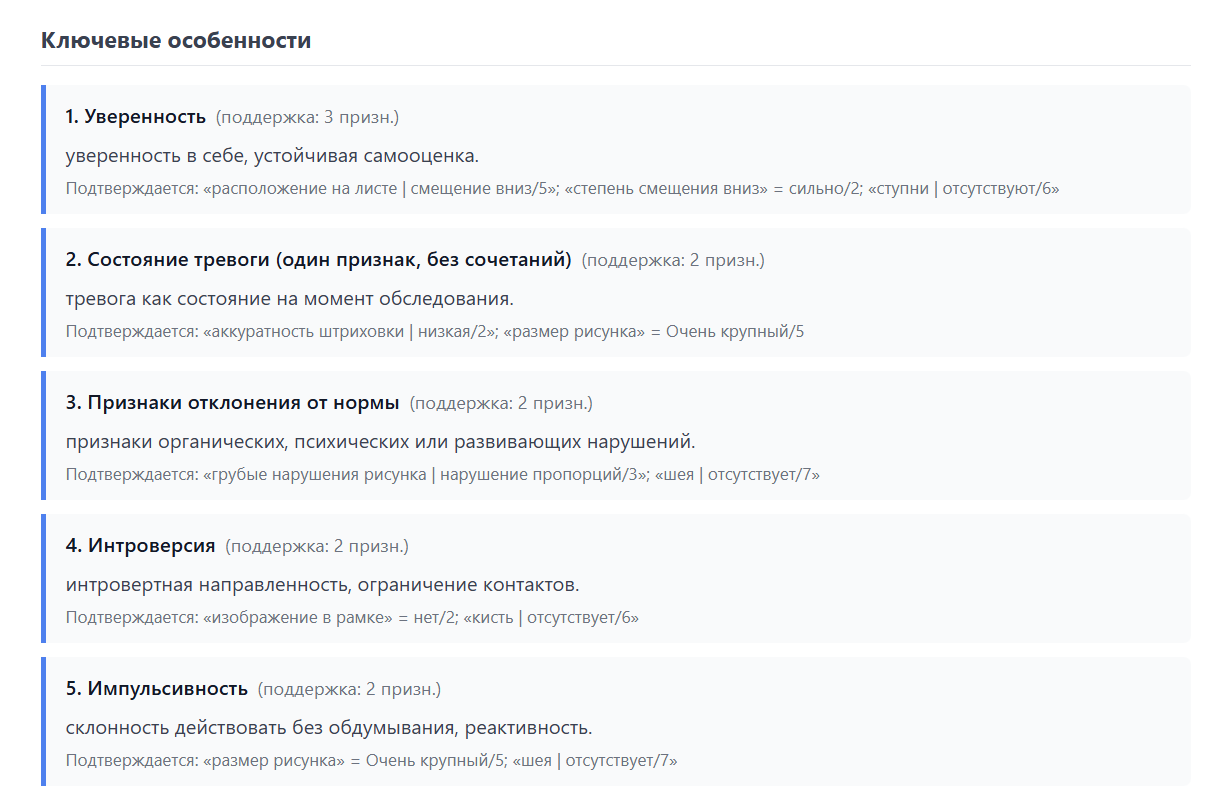
\includegraphics[width=0.8\linewidth]{inc/s2.png}
    \caption{Раздел <<Ключевые особенности>> сгенерированного психологического портрета}
    \label{fig:demo-traits}
\end{figure}

Помимо интерпретации, веб-интерфейс отображает технические детали работы модели. На рисунке~\ref{fig:demo-top10} приведена таблица десяти наиболее уверенных активных предсказаний с указанием имени признака, предсказанного значения и confidence (значение softmax).

\begin{figure}[h]
    \centering
    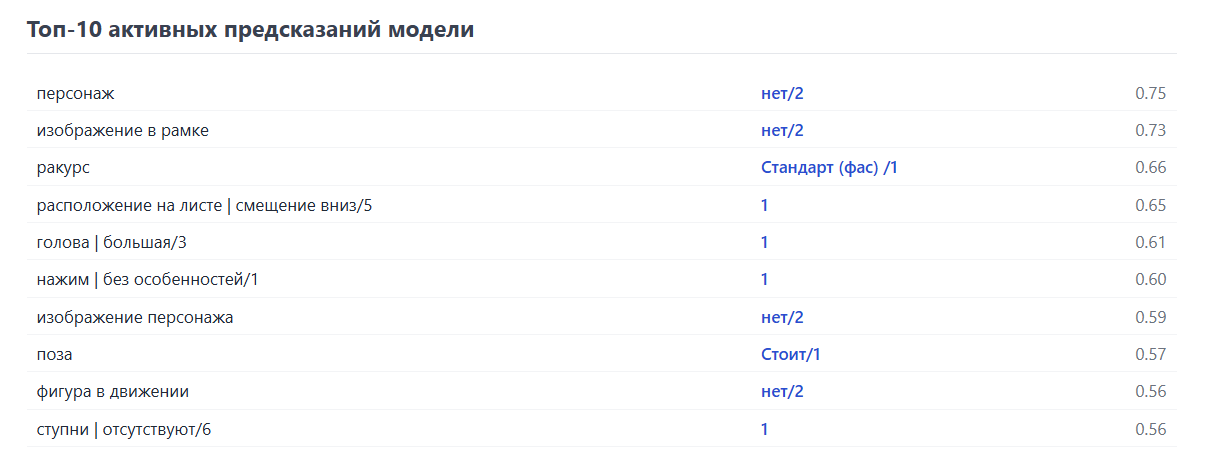
\includegraphics[width=0.8\linewidth]{inc/s3.png}
    \caption{10 активных предсказаний модели}
    \label{fig:demo-top10}
\end{figure}

\FloatBarrier
\subsection{Анализ временных характеристик}

Измерены характеристики времени работы программного комплекса в инференс-режиме на NVIDIA Tesla T4. Обработка одного рисунка от подачи на вход сырого изображения до возврата итогового текстового портрета занимает в среднем около 0,4~секунды. Это время разбивается на следующие компоненты:

\begin{itemize}
    \item чтение и декодирование изображения из файла --- около 0,05~с;
    \item локализация фигуры (адаптивная бинаризация, морфология, выделение связных компонент, фильтрация и объединение) --- около 0,15~с;
    \item кроп, паддинг, ресайз --- менее 0,01~с;
    \item инференс --- около 0,18~с (один прямой проход на одном изображении);
    \item декодирование 117 предсказаний и применение словаря интерпретаций --- менее 0,01~с;
    \item ранжирование черт и формирование итогового текста --- менее 0,01~с.
\end{itemize}

При пакетной обработке (batch inference) среднее время на один рисунок снижается за счёт лучшего использования параллелизма GPU: при обработке пакета из 32 рисунков время на одно изображение составляет около 0,05~секунд.

Время обучения модели от начала до завершения --- порядка 30--50~минут на одном NVIDIA Tesla T4 (50 эпох с ранней остановкой). Размер сохранённого чекпоинта --- около 22~МБ. Эти характеристики делают разработанный комплекс полностью применимым в практических условиях: при наличии современного GPU психолог может обработать пакет из сотен рисунков за несколько минут.

\subsection{Тестирование веб-сервиса}

Для верификации корректной работы микросервисной системы в целом проведено функциональное и нагрузочное тестирование развёрнутого веб-сервиса. Тестирование выполнялось на локальной машине (CPU: Intel Core i5, 16~ГБ ОЗУ) в режиме Docker-контейнеров без GPU.

Функциональное тестирование. Проверена корректность работы полного конвейера end-to-end: загрузка изображения через веб-форму, прохождение всех этапов обработки, формирование психологического портрета и сохранение результата в базу данных. Протестированы следующие сценарии:

\begin{itemize}
    \item загрузка типичного отсканированного рисунка формата A4 (2480$\times$3508, $\sim$1~МБ) --- успешная обработка, портрет сгенерирован;
    \item загрузка фотографии рисунка с мобильного устройства (4032$\times$3024, $\sim$3~МБ) --- успешная обработка;
    \item загрузка изображения без фигуры (чистый лист) --- система возвращает портрет без выраженных особенностей;
    \item загрузка файла некорректного формата --- корректная обработка ошибки с информативным сообщением;
    \item повторный просмотр сохранённого анализа по идентификатору --- портрет загружается из БД без повторного инференса.
\end{itemize}

Измерение времени отклика. Время обработки одного запроса (от отправки файла до получения HTML-портрета) при последовательной обработке составляет:

\begin{table}
    \caption{Время обработки одного рисунка через веб-сервис (CPU-режим)}
    \fontsize{12pt}{18pt}\selectfont
    \begin{tabular}{|l|c|}\hline
        \textbf{Этап} & \textbf{Время, с} \\ \hline
        Предобработка (OpenCV-локализация)    & 0,3--0,5 \\ \hline
        Вычисление bbox-признаков             & $<$\,0,01 \\ \hline
        Нейросетевой инференс (CPU)           & 1,5--2,5 \\ \hline
        Интерпретация и формирование портрета & $<$\,0,05 \\ \hline
        Сохранение в MinIO и PostgreSQL       & 0,1--0,2 \\ \hline
        Итого end-to-end                      & 2,0--3,2 \\ \hline
    \end{tabular}
    \label{tab:response-time}
\end{table}

Основное время занимает инференс на CPU. При развёртывании с GPU (NVIDIA Tesla T4) время инференса сокращается до $\sim$0,2~с, а общее время отклика --- до $\sim$0,7~с.

Нагрузочное тестирование. При параллельной отправке 10 запросов в секунду система обрабатывает все запросы без ошибок с линейным ростом латентности (запросы ставятся в очередь к единственному экземпляру сервиса инференса). При необходимости обслуживания большего числа одновременных пользователей достаточно горизонтально масштабировать сервис инференса (запуск нескольких реплик через Docker Compose).

Тестирование устойчивости. Проверена реакция системы на аварийные ситуации: при принудительной остановке контейнера \texttt{inference} API-шлюз возвращает корректное сообщение об ошибке; после перезапуска контейнера система восстанавливает работоспособность без ручного вмешательства благодаря директиве \texttt{restart: unless-stopped}. История ранее выполненных анализов остаётся доступной, поскольку хранится в PostgreSQL.

\subsection{Сфера применения и ограничения}

Разработанный программный комплекс может применяться психологами, педагогами и исследователями детской психологии в следующих сценариях.

Первый --- предварительный скрининг в детских садах и школах. Психолог может пропустить пакет рисунков через систему за минуты вместо часов и получить ранжированный список рисунков, требующих более детального индивидуального анализа.

Второй --- исследовательские задачи, в которых требуется обработка больших коллекций рисуночных тестов. Например, выявление средних тенденций в группе по полу или возрасту, корреляций психологических характеристик с социальными факторами, динамики изменения психологических черт со временем.

Третий --- учебные курсы по практической психологической диагностике. Система может применяться для демонстрации связи признаков рисунка с психологическими интерпретациями.

Среди ограничений разработки следует отметить следующие:

\begin{enumerate}
    \item система предназначена исключительно для теста <<Рисунок человека>> и не может быть напрямую применена к другим рисуночным тестам (<<Дом-Дерево-Человек>>, <<Несуществующее животное>>, <<Моя семья>> и др.) без переобучения. Возможна адаптация архитектуры для других тестов при наличии аналогичной обучающей выборки;
    \item выводы системы носят гипотетический характер и не могут заменить непосредственное общение специалиста с ребёнком, сбор анамнеза и наблюдение за ребёнком в естественных условиях. Психологический портрет, сгенерированный системой, является лишь предварительной гипотезой и должен подтверждаться независимыми источниками;
    \item точность предсказаний для редко встречающихся признаков объективно ограничена объёмом обучающих данных и требует осторожной интерпретации. Если итоговый портрет содержит черту, поддерживаемую только одним признаком, имеет смысл отнестись к ней с осторожностью; черты, поддерживаемые тремя и более признаками, существенно более надёжны;
    \item система обучена на рисунках детей дошкольного и младшего школьного возраста (приблизительно 5--12 лет). Для рисунков существенно других возрастных групп (подростков и взрослых) качество предсказаний может оказаться ниже, поскольку их рисуночные продукты имеют другие стилистические особенности;
    \item применение системы требует наличия отсканированного или сфотографированного рисунка достаточного качества. Сильно повреждённые, размытые или с фрагментированной фигурой изображения могут давать неустойчивые предсказания.
\end{enumerate}

Указанные ограничения не препятствуют практическому применению системы при учёте описанных условий и интерпретации её выводов как вспомогательных, а не окончательных.


    \conclusion

В результате выполнения выпускной квалификационной работы бакалавра был разработан программный комплекс автоматического распознавания визуальных признаков детских рисунков и сопоставления их с психологическими характеристиками ребёнка нейросетевыми методами. Были решены следующие задачи:

\begin{itemize}
    \item проведён анализ предметной области рисуночных тестов и существующих подходов к автоматизации их интерпретации;
    \item разработан собственный алгоритм предобработки изображений, реализующий локализацию фигуры человека на листе на основе классических операций обработки изображений (адаптивная бинаризация, морфологические операции замыкания, выделение связных компонент, фильтрация и объединение по якорной стратегии);
    \item спроектирована и обучена двухпотоковая собственная свёрточная нейросетевая модель (около 5,5\,млн параметров) для одновременной классификации 117 признаков рисунка;
    \item реализована стратегия обучения, устойчивая к сильному дисбалансу классов: взвешенная перекрёстная энтропия с насыщением весов классов, label smoothing для категориальных признаков, взвешенное случайное сэмплирование, групповое стратифицированное разбиение выборки;
    \item составлен словарь сопоставления 117 технических признаков с 26 каноническими психологическими чертами на основе методики А.~Л.~Венгера;
    \item реализован модуль генерации текстового психологического портрета с ранжированием черт по числу подтверждающих признаков;
    \item разработан микросервисный веб-сервис, объединяющий все модули в единый конвейер обработки с пользовательским интерфейсом, доступным через браузер;
    \item проведено экспериментальное исследование качества модели на тестовой выборке и функциональное тестирование веб-сервиса.
\end{itemize}

На тестовой выборке разработанная система достигла следующих показателей качества: F1\textsubscript{micro} = 0,901, F1\textsubscript{weighted} = 0,875, F1\textsubscript{macro} = 0,521. Значения F1\textsubscript{micro} и F1\textsubscript{weighted} означают, что модель корректно классифицирует около 90\,\% всех предсказаний по 117 признакам в совокупности. Заметно более низкое значение F1\textsubscript{macro} объясняется наличием в выборке нескольких признаков с экстремально малым числом положительных примеров (10 из 117 признаков имеют менее десяти положительных примеров в обучающей выборке), для которых надёжная классификация минорного класса принципиально невозможна без увеличения объёма данных.

Архитектурные особенности разработанного решения --- двухпотоковая модель, объединяющая визуальные признаки изображения и геометрические метаданные bounding box; раздельные проекционные головы для признаков различной сложности обучения; стратегия взвешенных потерь и взвешенного сэмплирования для обработки дисбаланса классов; собственный алгоритм локализации фигуры на основе классических методов обработки изображений --- обеспечивают качество классификации, достаточное для практического применения системы.

Для практического использования разработанные модули объединены в микросервисный веб-сервис, развёртываемый через Docker Compose. Архитектура включает шесть сервисов (предобработка, извлечение признаков, инференс, интерпретация, формирование отчёта, API-шлюз), базу данных PostgreSQL и объектное хранилище MinIO. Веб-интерфейс позволяет загрузить рисунок и получить психологический портрет за 2--3 секунды на CPU без необходимости установки локального окружения.

Программный комплекс автоматизирует рутинную часть обработки рисуночных тестов и позволяет психологу сосредоточиться на тех рисунках, которые требуют детального индивидуального анализа. Это особенно ценно при работе с большими коллекциями рисунков (групповое тестирование в детских садах, школах, исследовательские проекты).

Возможные направления развития работы включают:

\begin{itemize}
    \item расширение датасета редкими классами через целевой сбор рисунков с конкретными признаками, что повысит качество классификации редко встречающихся категорий;
    \item обучение отдельных специализированных моделей для самых сложных признаков по принципу per-criterion fine-tuning поверх общего бэкбона;
    \item применение более крупных архитектур и техник self-supervised предобучения на расширенной коллекции неразмеченных рисунков;
    \item расширение комплекса на другие рисуночные тесты (тесты <<Дом-Дерево-Человек>>, <<Несуществующее животное>>, <<Моя семья>>).
\end{itemize}

Исходный код разработанного программного комплекса размещён в открытом репозитории. QR-код для быстрого перехода к репозиторию приведён в приложении А на рисунке~\ref{fig:repo-qr}.

Полученный программный комплекс представляет собой цельное решение, в основе которого лежат современные методы глубокого обучения, классические алгоритмы обработки изображений, корректная инженерная работа с реальным несбалансированным датасетом и интеграция доменных психологических знаний. Результаты работы могут быть использованы как основа для дальнейших исследований и практических применений автоматизированной психологической диагностики на основе рисуночных тестов.


    \printbibliography

    \appendix
    \appendixsection{Исходный код}

QR-код на репозиторий с исходным кодом разработанного комплекса приведён на рисунке~\ref{fig:repo-qr}.

\begin{figure}[H]
    \centering
    
\includegraphics[width=0.3\linewidth,keepaspectratio]{inc/qr.png}
    \caption{QR-код на репозиторий с исходным кодом}
    \label{fig:repo-qr}
\end{figure}


\appendixsection{Архитектура нейросетевой модели}

\begin{figure}[H]
    \centering
    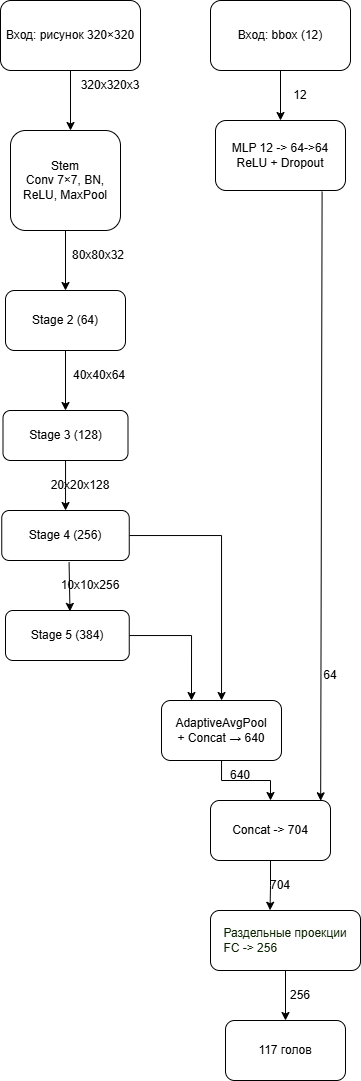
\includegraphics[width=0.35\linewidth,keepaspectratio]{inc/vkr.png}
    \caption{Архитектура нейросетевой модели}
    \label{fig:drawingnet-arch-appendix}
\end{figure}

\end{document}
